\documentclass{beamer}
\beamertemplatenavigationsymbolsempty
\usecolortheme{beaver}
\setbeamertemplate{blocks}[rounded=true, shadow=true]
\setbeamertemplate{footline}[page number]
%
\usepackage[utf8]{inputenc}
\usepackage[english]{babel}
\usepackage{amssymb,amsfonts,amsmath,mathtext}
\usepackage{subfig}
\usepackage[all]{xy} % xy package for diagrams
\usepackage{array}
\usepackage{multicol}% many columns in slide
\usepackage{hyperref}% urls
\usepackage{hhline}%tables
% Your figures are here:

%----------------------------------------------------------------------------------------------------------
\title{Using spatio-temporal dependencies to monitor additive manufacturing with deep learning}
\author[V.\,D.~Soldatov]{Vladislav Soldatov}
\institute{Moscow State University}
\date{\footnotesize
\par\smallskip\emph{Course:} My first scientific paper
\par\smallskip\emph{Expert:} Kropotov D.A.
\par\smallskip\emph{Consultant:} Sinilshchikov I.V.
\par\bigskip\small 2023}

%----------------------------------------------------------------------------------------------------------
\begin{document}
%----------------------------------------------------------------------------------------------------------
\begin{frame}
\thispagestyle{empty}
\maketitle
\end{frame}
%-----------------------------------------------------------------------------------------------------
\begin{frame}{Goal of research}
    Having an Additive Manufacturing setup, we need to ensure that it won't malfunction or produce defective pieces as a result of some oversight on the part of operators, which could be very possible in the cases with small details being printed and rapid laser movement.
    
    Therefore, it is of great importance to develop an algorithm that could momentarily spot anomalies during the printing process.
\end{frame}
%-----------------------------------------------------------------------------------------------------
% \begin{frame}{One-slide talk}

% The use of additive manufacturing in industry is currently limited due to the unknown in advance and unreliable quality of parts.

% \begin{columns}[c]
% \column{0.6\textwidth}

% \begin{figure}
%     \centering
%     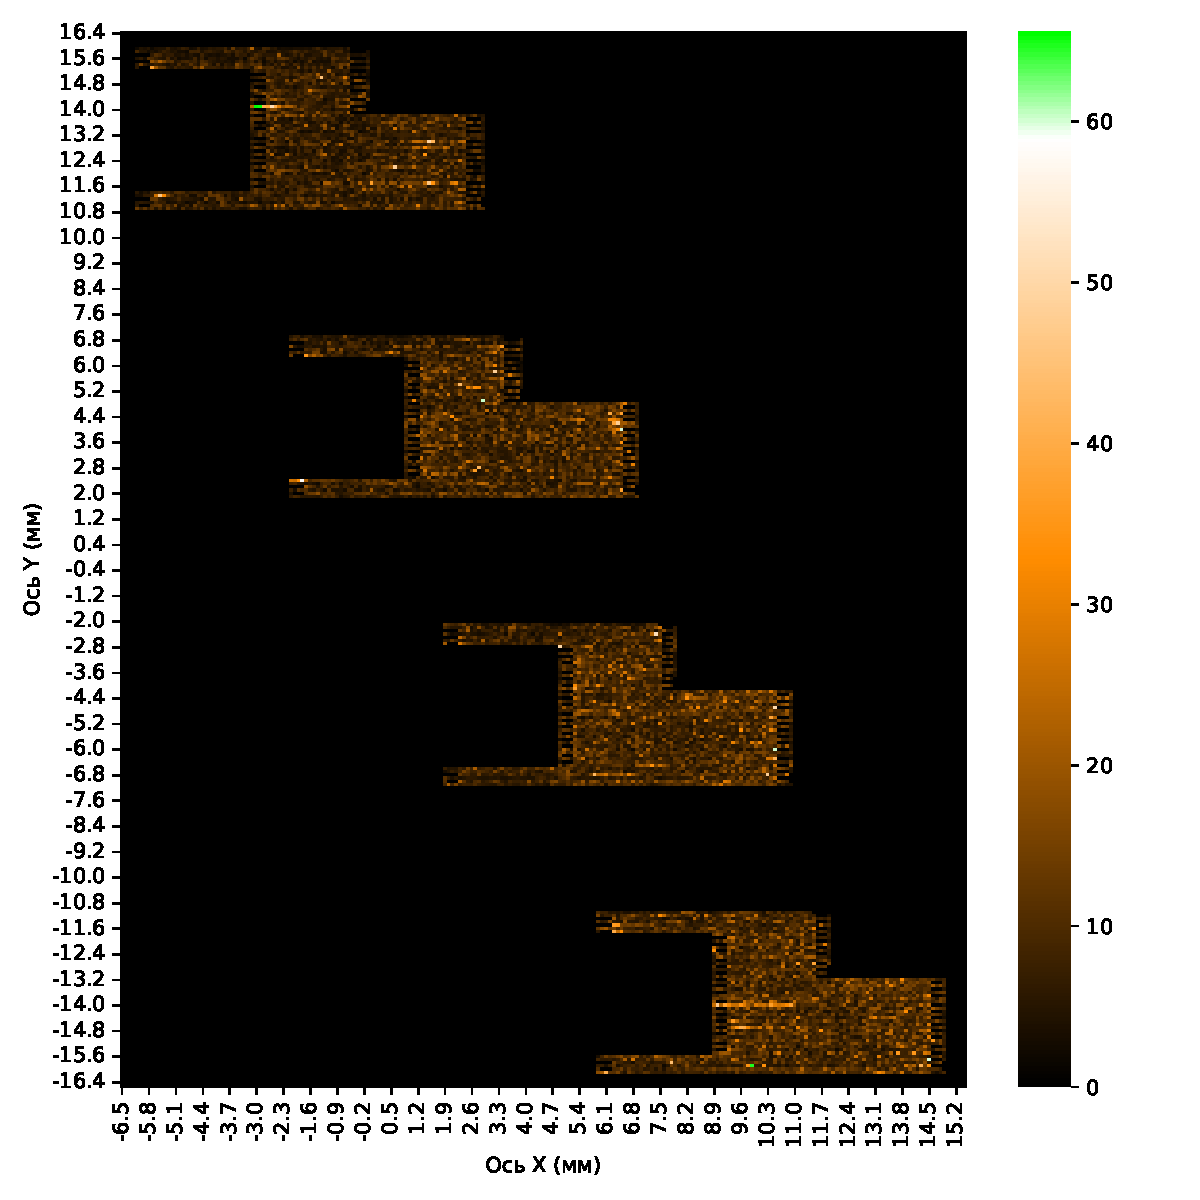
\includegraphics[scale=0.23]{lstm_4_window_xy_test_before.pdf}
%     \caption{Coordinate distribution of the error function for the ConvLSTMAE model.}
%     \label{fig:enter-label}
% \end{figure}
% \column{0.4\textwidth}
%     \textbf{Main task:} detect anomalous situations in AM processes on-line.

%     \textbf{Specifics:} given a sequence of meltpool frames, predict if laser will stumble across an obstacle at a certain point in time.
    
    %  This is largely caused by complex relationships between process parameters. Therefore, it is important to develop methods for monitoring AM processes in real time to ensure the quality of parts.

% \end{columns}

% \bigskip
% {\footnotesize {\color{red} Tags:} Additive manufacturing $\cdot{}$ Laser Powder Bed Fusion $\cdot{}$ Online monitoring $\cdot{}$ Flaw detection $\cdot{}$ Porosity prediction $\cdot{}$ Spatial-temporal Modeling}
% \end{frame}


%----------------------------------------------------------------------------------------------------------
\begin{frame}{Problem statement}
    To achieve the broadly stated goal, at least one manufacturing control system is needed. In this case, sequences of meltpool frames are used to detect any anomalous situations during the manufacturing process. This approach is called Laser Bed Power Fusion monitoring. Hence the training set is the following: $\mathbf{\mathcal{X}} = \{(\mathbf{X}_{1, 1}, \dots, \mathbf{X}_{1, m}), \dots (\mathbf{X}_{N, 1}, \dots, \mathbf{X}_{N, m})\}$, where $\mathbf{X}_{k, l}$ represents a matrix of intensity values captured with high-speed camera. Using the information extracted from those sequences, the algorithm must be able to determine which objects are the most unalike from the majority of training set. This is achieved with autoencoder models and a threshold on the values of quadratic loss between the sequence and its recreated version.
\end{frame}
%----------------------------------------------------------------------------------------------------------
\begin{frame}{Solution}
Two different possible models were chosen for the task:\vfill
\begin{columns}[c]
\column{0.46\textwidth}
    \textbf{ConvLSTMAE} is an autoencoder based on the LSTM model with matrix product operations swapped with convolutions. This enables the model to take value from both spatial and temporal dependencies in the data.
\column{0.54\textwidth}
    \textbf{UNET3d} model is inspired by great advances in the neighboring topic of motion recognition caused by the use of 3d-convolutions. It utilizes the well-known UNET autoencoder architecture with several adjustments including expanding the effective dimensionality of convolution filters
\end{columns}
\end{frame}
%----------------------------------------------------------------------------------------------------------
\begin{frame}{Computational experiment}
\begin{columns}[c]
\column{0.5\textwidth}
\begin{figure}
    \centering
    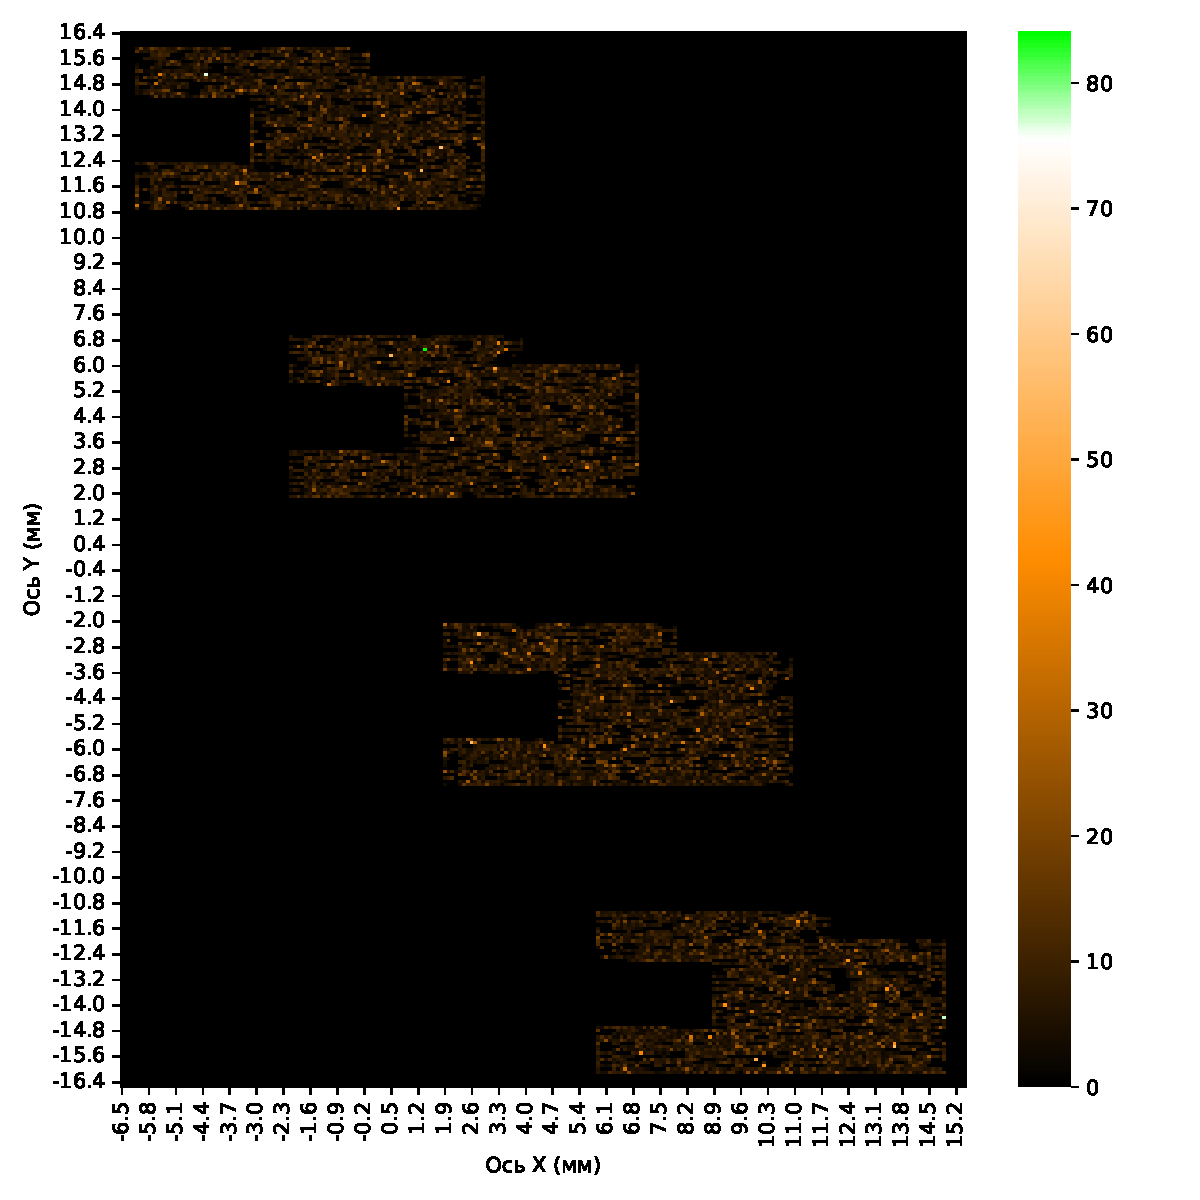
\includegraphics[scale=0.23]{lstm_4_window_xy_train_after.pdf}
    \caption{Coordinate distribution of the error function for the ConvLSTMAE model.}
    \label{convlstmae_xy}
\end{figure}

\column{0.5\textwidth}
\begin{figure}
    \centering
    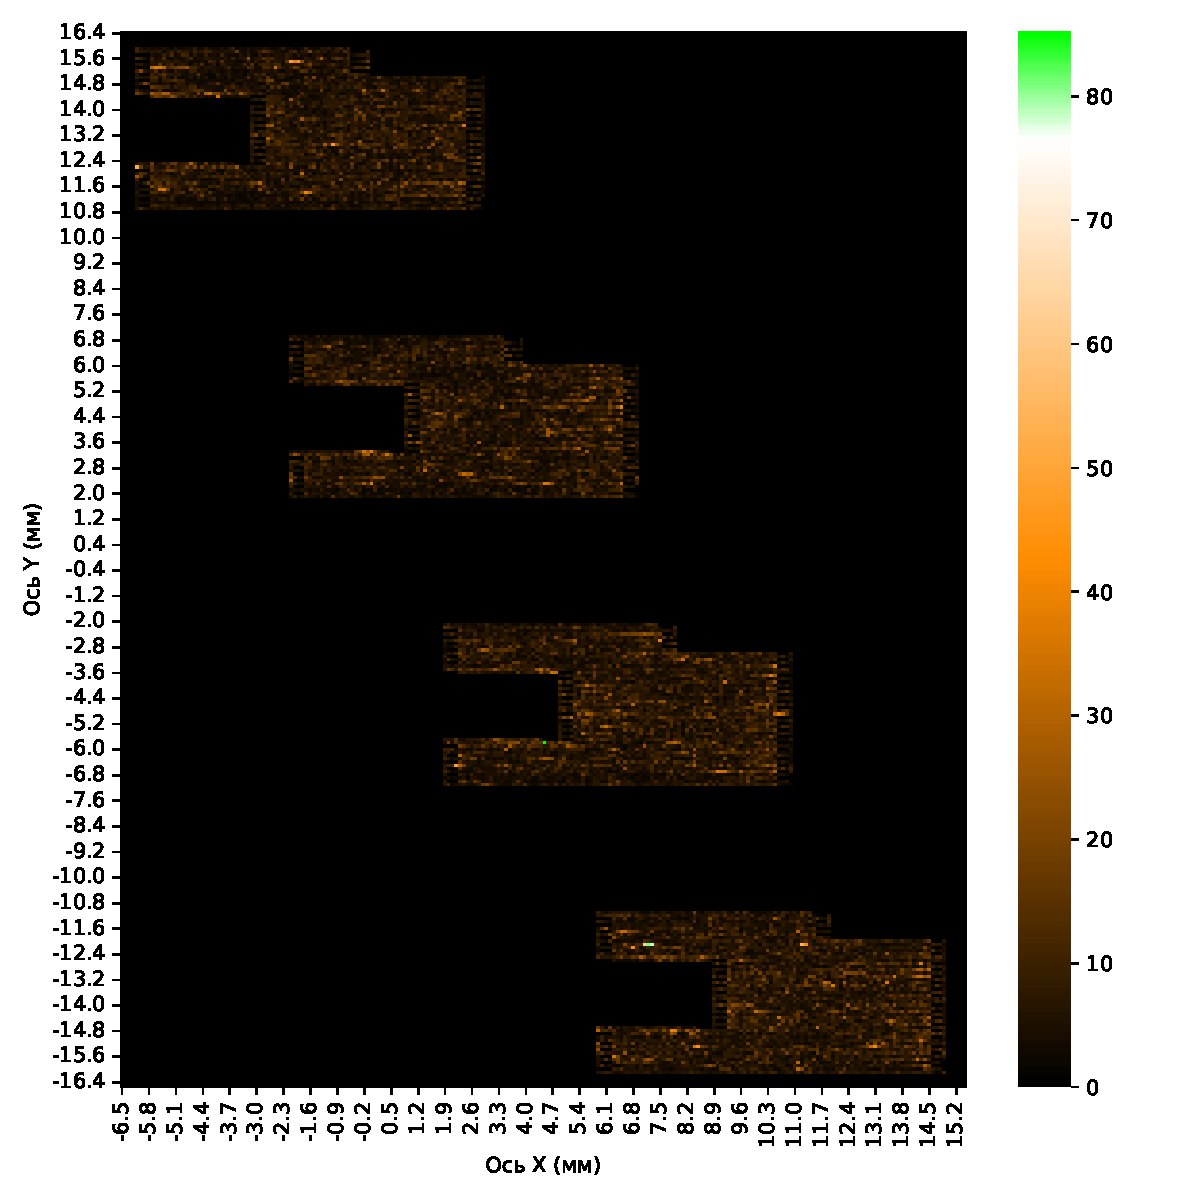
\includegraphics[scale=0.23]{unet_xy_train_after.pdf}
    \caption{Coordinate distribution of the error function for the UNET3d model.}
    \label{unet_xy}
\end{figure}
\end{columns}
\end{frame}

\begin{frame}{Computational experiment}
    \begin{table}[]
    \centering
    \begin{tabular}{|l||c|c|c|c|}
    \hline
    & PR-AUC & F1    & Precision & Recall \\ \hline\hline
    ConvLSTMAE & 0.516  & 0.638 & 0.750     & 0.556  \\ \hline
    UNET3d & 0.537  & 0.638 & 0.750     & 0.556  \\ \hline
    \end{tabular}
    \caption{Unbalanced learning-specific metrics for a small self-labelled part of the validation dataset.}
    \label{tab:sup_metrics}
    \end{table}
\end{frame}
%----------------------------------------------------------------------------------------------------------
\begin{frame}{Conclusion}
    \begin{block}{Immediate results}
        The research carried out in this work has shown that it is possible to use autoencoder models to simulate spatial and temporal dependencies in meltpool data and detect anomalous situations in the physical processes of laser melting. Experiments were conducted that showed a qualitative improvement when using the UNET3d model in the task under study.
    \end{block}
    
    \begin{block}{Future work}
        It is planned to build models capable of controlling laser power during the Additive Manufacturing processes based on reinforcement learning methods. This direction began to develop relatively recently, and researchers have already faced problems with the limited resources available for training and inferring neural networks during the additive printing process, which sets the goal to find less resource-intensive models with high computational speed, in the absence of quality losses.
    \end{block}
\end{frame}
%----------------------------------------------------------------------------------------------------------
\end{document} 